\chapter{Introduction}
\label{chp:introduction}

The sky



Mendeleev's periodic table is one 

Particle physicists are a group of people who are driven by the purest human
curiosity to devote their lives in the pursuit of ultimate reality for the
universe. Holding a belief that the world can be understood in terms of a few
fundamental building blocks, they have come up with a short list
of elementary particles that successfully assemble the visible world around us.
This list is usually known as the standard model in particle physics, including
twelve fermions that make up matter and a collection of force-carrying particles
to bond things together, usually referred to as bosons. A large series of
experiments have been performed to examine or fulfill the standard model during
the past decades, from which we have learned that it is the gluons that carry
the strong force and normally "glue" the quarks together into protons, neutrons
and, further, all the hard cores of the atoms making up the matter in our most
immediate environment. The theoretical and experimental impulse to describe the
properties and dynamics of quarks and gluons has led to the development of
quantum chromodynamics (QCD), which is a cornerstone to understand emergence of
nucleons and nuclei based on the constituent interactions.

Explore new land, path from nuclei to proton/neutron to partons. 

Rutherford bombarding a structure 

With the same footing of Rutherford, discovery of positron and neutron in
the 1930s opens a new gate to the 


Quark parton model is a remarkable achievement in the modern time physics 
to understand the hierarchy of our visible universe. The first hint shed
us a light on the possible underlying structure of nucleus emerges in the
1930s with the discovery of positron and neutron

Although past experiments were successful in determining the quark behavior in
the nucleon and light nuclei, the gluons that determine the essential features
of the strong interactions, remain largely unexplored. Of great interest is
especially, when the gluon density grows to a point where the self-interaction
of gluons have become so important that non-linear QCD effects supersede, a
phenomena named saturation. It is a universal behavior of gluons existing in any
hadronic systems ranging from pions, protons to nuclei. To date, it is still not
yet conclusive that such a saturated regime has been discovered at presently
running high energy experimental facilities. This pursuit will be facilitated by
the advent of a proposed high luminosity, high energy Electron-Ion Collider (EIC).


%With the ability to probe a large variety of nuclei species within a wide kinematics
%range on such a machine, we will be capable of unveiling the collective behavior
%of densely packed gluons in a strong color field deep into the saturation regime,
%essential to understand the origin of nuclear structure.
%


A theoretical framework is needed to translate the conceptual designs into a
quantitative analysis scheme. In the following sections, I will walk
through a general framework of gauge theory formulated to understand the
successive experimental results paving us the way to the fundamental constituents for our
universe.



\section{Quark Parton model and Deep inelastic scattering}\label{sec:basicQCD}
By the time of 1960s, people have discovered a large range of hadrons 
in various experiments. And reactions following certain conservation laws
may convert one type of hadron to another type. Analysis performed on these 
conservation laws and the properties of these hadrons indicates that
there exists some common substructure that forms all the hadronic objects ranging
from pions to protons or neutrons.


Suggested by Gell-Mann and Zweig in 1964, a group of point-like
particles named by quarks 
can be used to describe this fundamental substructures that build up the hadron hierarchy. 
For instance, in the naive picture, a proton is made up of two ``up" quarks and one ``down" quark. 
These quarks are supposed to be fermions with fractional charge following SU3 symmetry. Due to the color confinement feature of strong force, there is no isolated fractional electric
charge ever seen in a detector. However, although it is impossible to directly detect these elementary
constituents, one can still obtain the their information with the
structureless lepton probes bombarding hadrons similar to the strategies of ``Rutherford-prime" experiment.

This type of study was firstly performed at the Standford Linear Accelerator Center (SLAC) experiment with 20 GeV electron beams
bouncing off proton target. 
The electron proton scattering process performed at this experiment can be
illustrated by Fig.~\ref{fig:DIS_kinematics} with the notation of
\( e(k)+proton(P) \rightarrow e^{\prime}(\kp) + X, \)
where $X$ represents any hadronic final systems allowed by conservation laws.
The process is mediated by a virtual vector boson, with 4-momentum given by $q=k-\kp$.

\begin{figure}
\centering
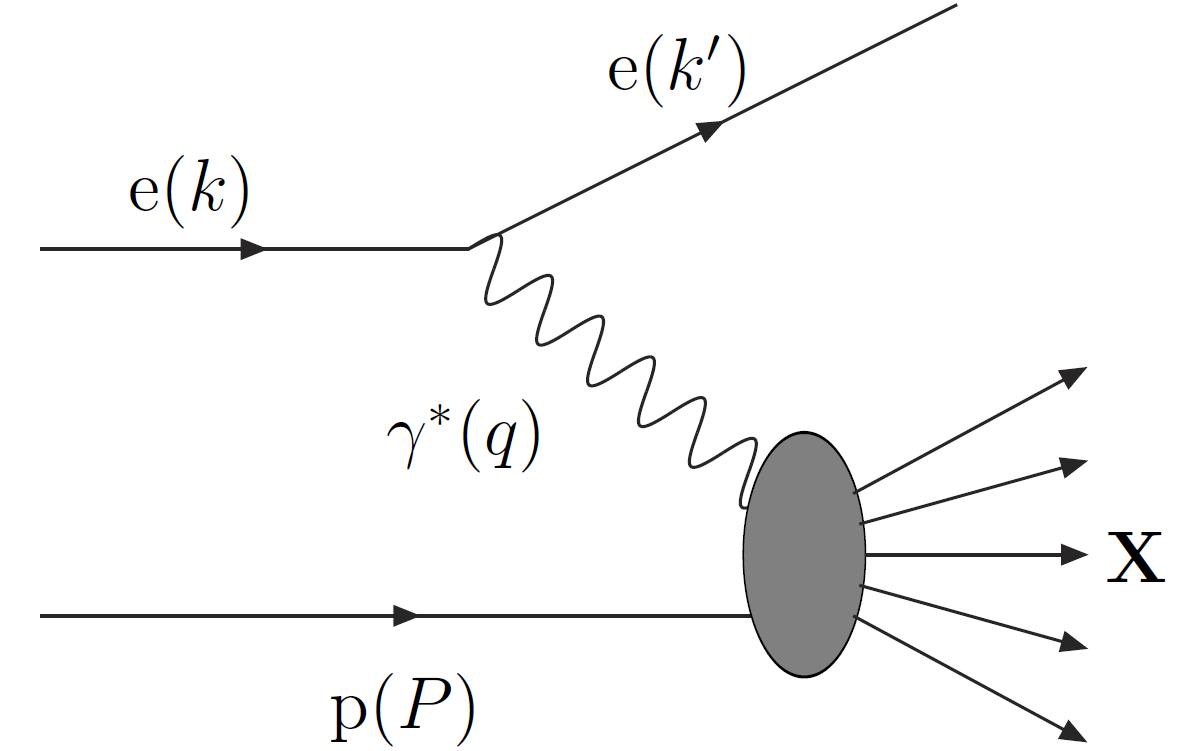
\includegraphics[width=0.5\textwidth]{plots/chpt1/DIS_kinematics.png} 
\caption[DIS scattering diagram] {
Schematic diagram of DIS scattering via virtual photon exchange.
\label{fig:DIS_kinematics}
}
\end{figure}

The selection of Lorentz invariant variables describing Fig.~\ref{fig:DIS_kinematics} is only a matter of convention,
but the following set of the kinematics variables is commonly used:

\begin{align}
s = (k+P)^{2}, \\
Q^{2} = -q^{2} = -(k-\kp)^{2}, \\
x_{Bj} = \frac{Q^{2}}{2P\cdot q}, \\
y = \frac{P\cdot q}{ P\cdot k}, \\
\nu = \frac{P\cdot q}{ M_{p} }, \\
W^{2} = (P+q)^{2},
\end{align}
in which $s$ is the center-of-mass (CM) energy squared for \ep\ interaction;
$Q^{2}$ measures the magnitude of momentum transfer mediated by the virtual
boson, at intermediate $Q^{2}$ only photon exchange needs to be considered;
$x_{Bj}$ is the Bjorken $x$, which can be interpreted as momentum fraction of
struck quark taken from the incoming nucleon in the quark parton model; $y$ is
named as the inelasticity, giving fraction of the electron energy transfered to
the hadronic system; $\nu$ suggests the energy current from lepton in the proton
rest frame; and the invariant mass of the final state hadronic system is often
denoted by $W$.


With large momentum transfer \qsq, we are allowed to resolve smaller objects
having transverse momenta less than $Q$ and localized within a transverse
area $\sim 1/Q^{2}$. The regime of $Q^{2}\geq$ 1 \gevsq\ is often referred
to as the DIS regime, in which one can directly deduce the composite objects
of the proton. 



Analysis about the distribution for the scattered electron shows a strong scaling
behavior, 
As suggested by Bjorken, a scaling effect is observed in the results from
this measurement. 

The parton model was first introduced by Feynman to interpret the 
scaling behavior observed in the SLAC data. The basic assumption
of this parton model is to represent the electron proton scattering
as incoherent sum of scatterings on some individual point-like constituents 
within the proton called partons.




\section{From parton model to QCD}

\subsection{Asymptotic Freedom}

\subsection{Formation of hadronic object}

\section{Factorization and evolutions}\label{sec:DIS}

\subsection{Parton Distribution Function}

\subsection{Evolution of Parton Distributions}\label{sec:PDFevo}


